\documentclass[conference,onecolumn]{IEEEtran}
\IEEEoverridecommandlockouts
% The preceding line is only needed to identify funding in the first footnote. If that is unneeded, please comment it out.
\usepackage{cite}
\usepackage{amsmath,amssymb,amsfonts}
\usepackage{algorithmic}
\usepackage{graphicx,subcaption}
\usepackage{float}
\usepackage{hyperref}
\usepackage{textcomp}
\usepackage{xcolor}
\usepackage{listings}
\usepackage{enumitem}

\DeclareMathOperator*{\argmax}{arg\,max}
\DeclareMathOperator*{\argmin}{arg\,min}

\def\BibTeX{{\rm B\kern-.05em{\sc i\kern-.025em b}\kern-.08em
    T\kern-.1667em\lower.7ex\hbox{E}\kern-.125emX}}

\IEEEoverridecommandlockouts

\lstset{
    language=MATLAB,             % Set language to MATLAB
    basicstyle=\ttfamily\small,  % Set font to small and monospaced
    keywordstyle=\color{blue},   % Color keywords
    stringstyle=\color{green},   % Color strings
    commentstyle=\color{gray},   % Color comments
    showstringspaces=false,      % Do not display string spaces
    frame=single,                % Add a frame around the code
    breaklines=true              % Line breaks for long lines
}

\begin{document}

\title{\Large Assignment 2 --- Math Fundamentals for Robotics 16-811, Fall 2024}

\author{
    \IEEEauthorblockN{Mukai Yu}
    \IEEEauthorblockA{\textit{MSR, CMU} \\
        Pittsburgh, PA\\
        \href{mailto:mukaiy@andrew.cmu.edu}{mukaiy@andrew.cmu.edu}}
}

\maketitle

\begin{enumerate}[label=\arabic{enumi}.]
    \item \begin{enumerate}
              \item Implement a procedure that interpolates $f(x)$ based on a divided difference approach.

                    The procedure should take as input the following parameters:
                    $$
                        x, x_0, ... , x_n, f(x_0), ... , f(x_n) (\text{with distinct } x_0, x_1, ... , x_n).
                    $$
                    The procedure should compute an interpolated value for $f(x)$ based on the given data points $(x_0, f(x_0))$, $(x_1, f(x_1))$, ... , $(x_n, f(x_n))$.

                    Note: The procedure should use all the data points $(x_i, f(x_i)), i = 0, ... , n$, effectively implementing an interpolating polynomial of degree n (or less, depending on the data).

                    \textbf{Solution:}

                    \begin{lstlisting}[language=MATLAB]
function polynomial_interpolation = divided_difference(X, F)
    % divided_difference constructs the interpolating polynomial
    % using Newton's Divided Difference method and returns the symbolic function.
    %
    % Inputs:
    %   X  - vector containing the x values: [x0, x1, ..., xn]
    %   F  - vector containing the corresponding function values: [f(x0), f(x1), ..., f(xn)]
    %
    % Output:
    %   polynomial_interpolation - the symbolic function representing the interpolating polynomial

    % Assert that X and F are of the same length
    assert(length(X) == length(F), 'X and F must have the same length.');

    syms x; % Define symbolic variable for x
    n = length(X); % Number of data points
    diff_table = zeros(n, n); % Initialize the divided difference table

    % Fill the first column with the function values
    diff_table(:, 1) = F(:); % Column vector of function values

    % Compute the divided differences
    for j = 2:n

        for i = 1:n - j + 1
            diff_table(i, j) = (diff_table(i + 1, j - 1) - diff_table(i, j - 1)) / (X(i + j - 1) - X(i));
        end

    end

    % Construct the interpolating polynomial symbolically
    polynomial_interpolation = diff_table(1, 1); % The first term (f(x0))
    product_term = 1; % To hold the product of (x - x0), (x - x1), ...

    for k = 2:n
        product_term = product_term * (x - X(k - 1)); % (x - x0)(x - x1)...(x - x(k-2))
        polynomial_interpolation = polynomial_interpolation + diff_table(1, k) * product_term;
    end

    % Simplify the polynomial
    polynomial_interpolation = simplify(polynomial_interpolation);
end
                    \end{lstlisting}
              \item use your procedure to interpolate $cos(\pi x)$ at $x = \frac{3}{10}$, based on known values of $(x, cos(\pi x))$ at the following x locations: $0, \frac{1}{8}, \frac{1}{4}, \frac{3}{8}, \frac{1}{2}$.

                    \textbf{Solution:}

                    \begin{align*}
                        p(\frac{3}{10}) \approx \frac{42359543354865945937}{72057594037927936000} = 0.5878567543147465
                    \end{align*}
              \item Now consider the function
                    $$
                        f(x) = \frac{2}{1 + 9x^2},
                    $$
                    with input data given at the points
                    $$
                        x_i = i \frac{2}{n} - 1, i = 0, ... , n.
                    $$
                    Use your procedure to estimate $f(x)$ at $x = 0.07$, with $n = 2$.

                    Use your procedure to estimate $f(x)$ at $x = 0.07$, with $n = 4$.

                    Use your procedure to estimate $f(x)$ at $x = 0.07$, with $n = 40$.

                    What is the actual value of $f(0.07)$?

                    \textbf{Solution:}
                    \begin{align*}
                        p_2(x)    & = 2 - \frac{9}{5}x^2 = 2 - 1.8x^2                                                   \\
                        p_4(x)    & = 2 - \frac{441}{65}x^2 + \frac{423}{65}x^4 \approx 2 - 6.7846x^2 + 4.9846x^4       \\
                        p_{40}(x) & \approx 2 + 1.8871 \times 10^{-15}x - 18 x^2 + \ldots + 1.0512 \times 10^{+9}x^{40}
                    \end{align*}

                    Refer to my \textit{divided\_difference.ipynb} for the full form of $p_{40}$.
                    \begin{align*}
                        p_2(0.07)    & = \frac{99559}{50000} = 1.99118                            \\
                        p_4(0.07)    & = \frac{3196171981}{1625000000} = 1.9668750652307692       \\
                        p_{40}(0.07) & \approx  1.9155253271352064                                \\
                        f(0.07)      & = \frac{2}{1 + 9 \times 0.07^2} \approx 1.9155253328225266
                    \end{align*}
              \item In this part, you are to (numerically) estimate the maximum interpolation error
                    $$
                        E_n = \max_{-1 \leq x \leq 1} |f(x) - p_n(x)|.
                    $$
                    (You don't need to do anything fancy; simply discretize the interval [-1, 1] very finely - much more finely than the discretization implied by n.
                    Then compute errors at the resulting discrete points.)

                    Estimate $E_n$ for $n = 2, 4, 6, 8, 10, 12, 14, 16, 18, 20$, and $40$, for the function $f(x) = \frac{2}{1 + 9 x^2}$ given above and $p_n(x)$ the interpolating polynomial based on n using data as in part (c).

                    Do the error estimates make sense? Explain your results.

                    \textbf{Solution:}

                    For each n, evenly discretize the interval [-1, 1] into $100 \times n$ points, then max among these points.
                    \begin{align*}
                        E_2    & \approx 0.9350888158435888 \\
                        E_4    & \approx 0.596313372781065  \\
                        E_6    & \approx 0.6301901751946674 \\
                        E_8    & \approx 0.7681245303002563 \\
                        E_{10} & \approx 0.9995971865664737 \\
                        E_{12} & \approx 1.3514858830490715 \\
                        E_{14} & \approx 1.8739160198479834 \\
                        E_{16} & \approx 2.6450175325958294 \\
                        E_{18} & \approx 3.783412922067518  \\
                        E_{20} & \approx 5.4696283033072435 \\
                        E_{40} & \approx 290.8113085542939
                    \end{align*}

                    The error estimates make sense because too many data points or too high degree of interpolating function lead to overfitting, which results in a higher maximum error.
          \end{enumerate}
          \clearpage
    \item Suppose you wish to build a “sliding-window interpolation table” (as discussed in class) with entries of the form $(x, f(x))$ for the function $f(x) = sin x$ over the interval $[0, 2\pi]$.
          Please use uniform spacing between points.
          How fine must the table spacing be in order to ensure 6 decimal digit $\text{accuracy}^1$, assuming that you will use linear interpolation between adjacent points in the table?
          How fine must the table spacing be if you will use quadratic interpolation?
          In each case, how many entries do you need in the table?

          \textbf{Solution:}

          \begin{lstlisting}[language=MATLAB]
function min_interval = interpolation_interval(f, range, degree, error_tolerance)
    % interpolation_interval finds the minimum interval that satisfies the error tolerance to interpolate f with given degree of polynomial function.
    %
    % Inputs:
    %   f              - the function to interpolate
    %   range          - the range of x values: [a, b]
    %   degree         - the degree of the interpolating polynomial
    %   error_tolerance - the maximum error tolerance
    %
    % Output:
    %   min_interval - the minimum interval that satisfies the error tolerance

    syms x real; % Define symbolic variable for x

    f_sym = str2sym(f);

    % Derive coefficient function
    coefficient_function = diff(f_sym, x, degree + 1) / factorial(degree + 1);

    % Find the maximum value of the coefficient function in the range
    coefficient_function_handle = matlabFunction(-coefficient_function);
    max_coefficient_x = fminbnd(@(x) coefficient_function_handle(x), range(1), range(2));

    max_coefficient = subs(coefficient_function, max_coefficient_x);

    syms y h real;
    assumeAlso(h > 0 & h < 1);
    assumeAlso(y >= 0 & y <= degree * h);

    % Construct the error bound function
    error_bound_function = max_coefficient;

    for i = 0:degree
        error_bound_function = error_bound_function * (y - i * h);
    end

    error_bound_function = simplify(abs(error_bound_function));

    disp("error_bound_function:")
    disp(vpa(error_bound_function, 5));

    % Get the maximum expression of error_bound_function with y in range [0, degree * h] and h as positive constant
    % Can assume h will not be greater than 1
    % Resulting in a function with only h as variable
    derror_dy = diff(error_bound_function, y);

    disp("derror_dy:")
    disp(vpa(derror_dy, 5));

    critical_points = solve(derror_dy == 0, y, "Real", true);
    critical_points = critical_points(isAlways(critical_points >= 0 & critical_points <= degree * h));
    candidate_points = [0; critical_points; degree * h];

    disp("candidate_points:")
    disp(candidate_points);

    error_bound_function_values = subs(error_bound_function, y, candidate_points);

    % Find the maximum value and corresponding y
    max_error_bound_function = simplify(max(error_bound_function_values));

    disp("max_error_bound_function:")
    disp(vpa(max_error_bound_function, 5));

    % Solve for max_error_bound_function = error_tolerance / 2
    min_interval = solve(max_error_bound_function == (error_tolerance / 2), h, "Real", true);

end
          \end{lstlisting}
          It did not work in cubic or quartic interpolation as expected, possibly due to imaginary roots.
          \begin{enumerate}
              \item Linear Interpolation:

                    The error function is:
                    \begin{align*}
                        e_1(\bar{x}) & = \frac{f''(\xi)}{2!}(\bar{x} - x_{i})(\bar{x} - x_{i+1})                                \\
                                     & \leq \max_{0 \leq x \leq 2 \pi} |\frac{f''(x)}{2!}| (\bar{x} - x_{i})(\bar{x} - x_{i+1}) \\
                                     & = \max_{0 \leq x \leq 2 \pi} |-\frac{sin(x)}{2}| (\bar{x} - x_{i})(\bar{x} - x_{i+1})    \\
                                     & = \frac{1}{2} (\bar{x} - x_{i})(\bar{x} - x_{i+1})                                       \\
                                     & \leq \max_{0 \leq y \leq h} \frac{1}{2} |y(y + h)|                                       \\
                    \end{align*}
                    Where $y = \bar{x} - x_{i}$ and $h = x_{i+1} - x_i$.
                    Let $g(y) = \frac{1}{2} |y(y - h)|$ for $y \in [0, h]$, then $g'(y) = - y + \frac{1}{2}h$.
                    So the maximum of $g(y)$ is at $y = \frac{1}{2}h$, $g(\frac{1}{2}h) = \frac{1}{8}h^2$.

                    Thus
                    \begin{align*}
                        e_1(\bar{x}) \leq \frac{1}{8} h^2 & \leq 5 \times 10^{-7}                                       \\
                        h                                 & \leq \sqrt{40 \times 10^{-7}} \approx 0.0020000000000022066
                    \end{align*}
                    Then we need $\frac{2\pi}{h} + 1 \approx 3142.592653586327 \approx 3143$ entries in the table.
              \item Quadratic Interpolation:
                    The error function is:
                    \begin{align*}
                        e_1(\bar{x}) & = \frac{f'''(\xi)}{3!}(\bar{x} - x_{i-1})(\bar{x} - x_i)(\bar{x} - x_{i+1})                                  \\
                                     & \leq \max_{0 \leq x \leq 2 \pi} |\frac{f'''(x)}{3!}| (\bar{x} - x_{i-1})(\bar{x} - x_{i})(\bar{x} - x_{i+1}) \\
                                     & = \max_{0 \leq x \leq 2 \pi} |-\frac{cos(x)}{6}| (\bar{x} - x_{i-1})(\bar{x} - x_{i})(\bar{x} - x_{i+1})     \\
                                     & = \frac{1}{6} (\bar{x} - x_{i-1})(\bar{x} - x_{i})(\bar{x} - x_{i+1})                                        \\
                                     & \leq \max_{-h \leq y \leq h} \frac{1}{6} |(y - h)y(y + h)|                                                   \\
                    \end{align*}
                    Where $y = \bar{x} - x_{i}$ and $h = x_{i+1} - x_i$.
                    Let $g(y) = \frac{1}{6} |(y - h)y(y + h)|$ for $y \in [-h, h]$, then $g'(y) = \frac{1}{6}(3y^2 - h^2)$.
                    So the maximum of $g(y)$ is at $y = \frac{1}{\sqrt{3}}h$, $g(\frac{1}{\sqrt{3}}h) = \frac{1}{6} \cdot \frac{2}{3} \cdot \frac{1}{\sqrt{3}} h^3$.

                    Thus
                    \begin{align*}
                        e_1(\bar{x}) \leq \frac{1}{9\sqrt{3}}h^3 & \leq 5 \times 10^{-7}                                                \\
                        h                                        & \leq \sqrt[3]{45\sqrt{3} \times 10^{-7}} \approx 0.01982703228250094
                    \end{align*}
                    Then we need $\frac{2\pi}{h} + 1 \approx 317.8999383092263 \approx 318$ entries in the table.
          \end{enumerate}

          \clearpage
    \item Implement Newton's Method. Consider the following equation:
          $$
              x = tan x.
          $$
          There are an infinite number of solutions x to this equation.
          Use Newton's method to find the two solutions on either side of 15.
          In other words, find two solutions $x_{low} < 15 < x_{high}$ such that the interval $[x_{low}, x_{high}]$ contains no other solutions. — Use any techniques you need to start Newton in regions of convergence.
          Those regions may be very small.

          \textbf{Solution:}

          \begin{lstlisting}[language=MATLAB]
function root = newton_method(f, x0, tol, max_iter)
    % Initialize variables
    syms x real;

    f = str2sym(f);
    df = diff(f, x);

    f_handle = matlabFunction(f);
    df_handle = matlabFunction(df);

    disp("f_handle:")
    disp(f_handle);
    disp("df_handle:")
    disp(df_handle);

    x_current = double(x0);
    iter = 0;
    % Loop until the maximum number of iterations is reached
    while iter < max_iter
        % Calculate the derivative of the function at x
        % Calculate the next approximation of the root using Newton's method
        x_next = x_current - f_handle(x_current) / df_handle(x_current);
        % Check if the absolute difference between the current and next approximation is less than the tolerance
        if abs(f_handle(x_next)) < tol
            root = x_next;
            disp("Preliminary stop at iteration: " + iter);
            return;
        end

        % Update the current approximation and iteration count
        x_current = x_next;
        iter = iter + 1;
    end

    % If the maximum number of iterations is reached, return the current approximation
    root = x_current;
end
          \end{lstlisting}
          $$
              [x_{low}, x_{high}] \approx [14.066193915002767, 17.220755272066615]
          $$

          \clearpage
    \item Suppose $\xi$ is a root of order 2 of $f(x)$, meaning $f(\xi) = 0, f'(\xi) = 0$ and $f''(\xi) \neq 0$.
          \begin{enumerate}
              \item Show that in this case Newton's method no longer converges quadratically.
                    Do so by showing that the method now converges linearly.

                    \textbf{Solution:}

                    Let $h(x) = \frac{f(x)}{f'(x)}$, then
                    \begin{align*}
                        h(\xi)  & = \frac{f(\xi)}{f'(\xi)} = \frac{f'(\xi)}{f''(\xi)} = 0,                                                      \\
                        h'(\xi) & = 1 - \frac{f(\xi)f''(\xi)}{f'(\xi)^2}                                                                        \\
                                & = 1 - \frac{f'(\xi)f''(\xi) + f(\xi)f'''(\xi)}{2f'(\xi)f''(\xi)}                                              \\
                                & = \frac{1}{2} - \frac{f(\xi)f'''(\xi)}{2f'(\xi)f''(\xi)}                                                      \\
                                & = \frac{1}{2} - \frac{1}{2} \cdot \frac{f'(\xi)f'''(\xi) + f(\xi)f^{(4)}(\xi)}{f''(\xi)^2 + f'(\xi)f'''(\xi)} \\
                                & = \frac{1}{2}
                    \end{align*}
                    Thus
                    \begin{align*}
                        h(\xi + \epsilon) & = h(\xi) + \epsilon h'(\xi) + \frac{\epsilon^2}{2}h''(\xi) + \ldots \\
                                          & = 0 + \frac{1}{2}\epsilon + \frac{\epsilon^2}{2}h''(\xi) + \ldots
                    \end{align*}
                    Where $\epsilon_n = \xi - x_n$, $\epsilon_n$ denotes the error of $x_n$ to the true root $\xi$.
                    Thus $x_n = \xi - \epsilon_n$

                    For vanilla Newton's method, we have
                    \begin{align*}
                        x_{n+1}              & = x_n - \frac{f(x_n)}{f'(x_n)} = x_n - h(x_n)                                  \\
                        \xi - \epsilon_{n+1} & = \xi - \epsilon_n - h(\xi - \epsilon_n)                                       \\
                        - \epsilon_{n+1}     & = \epsilon_n - \frac{1}{2}\epsilon_n - \frac{\epsilon_n^2}{2}h''(\xi) - \ldots \\
                        |\epsilon_{n+1}|     & \sim \frac{1}{2}|\epsilon_n|
                    \end{align*}
                    Thus
                    \begin{align*}
                        \lim_{n \to \infty} \frac{|\epsilon_{n+1}|}{|\epsilon_n|} = \frac{1}{2}
                    \end{align*}
                    And the method converges linearly.

              \item We can modify Newton's method in this case: Show that the iteration
                    $$
                        x_{n+1} = x_n - 2 \frac{f(x_n)}{f'(x_n)}
                    $$
                    does converge quadratically (or faster) when $\xi$ is a root of order 2 of $f(x)$.

                    Throughout this problem you may assume that $f(x)$ has as many continuous derivatives as you need, for instance that $f'''(x)$ is continuous in a neighborhood of $\epsilon$.

                    \textbf{Recommendation:} Use a Taylor series for $h(x) = \frac{f (x)}{f'(x)}$, similar to what we did in lecture when examining convergence of Newton's method.
                    You do not need anything more complicated.
                    However, you will find it useful to remember L'Hopital's rule from calculus when computing $h(\epsilon)$ and $h'(\epsilon)$.
                    Do not worry about the exact value of $h''(\xi)$.

                    \textbf{Solution:}

                    Similarly,
                    \begin{align*}
                        x_{n+1}              & = x_n - 2\frac{f(x_n)}{f'(x_n)} = x_n - 2h(x_n)           \\
                        \xi - \epsilon_{n+1} & = \xi - \epsilon_n - 2h(\xi - \epsilon_n)                 \\
                        - \epsilon_{n+1}     & = \epsilon_n - \epsilon_n - \epsilon_n^2h''(\xi) - \ldots \\
                        - \epsilon_{n+1}     & = - \epsilon_n^2h''(\xi) - \ldots                         \\
                    \end{align*}
                    Thus
                    \begin{align*}
                        \lim_{n \to \infty} \frac{|\epsilon_{n+1}|}{|\epsilon_n|^2} = |h''(\xi)|
                    \end{align*}
                    And the method converges quadratically.
          \end{enumerate}

          \clearpage
    \item
          \begin{enumerate}
              \item Implement Muller's method.

                    \textbf{Solution:}
                    \begin{lstlisting}[language=Python]
def divided_difference_table(X: np.ndarray, Fx: np.ndarray) -> np.ndarray:
    """Construct divided difference table

    Args:
        X (np.ndarray): vector of x values
        Fx (np.ndarray): vector of f(x) values

    Returns:
        np.ndarray: divided_difference_table with columns indicating # of x values used, rows indicating leading x index
    """

    X = X.copy().astype(complex).reshape(-1)
    Fx = Fx.copy().astype(complex).reshape(-1)

    assert X.shape == Fx.shape, "X and F must have the same length!"

    n = X.shape[0]

    divided_difference_table = np.zeros((n, n)).astype(complex)
    divided_difference_table[:, 0] = Fx.reshape(-1, 1)[:, 0]

    for column in range(1, n):
        for row in range(0, n - column):
            divided_difference_table[row, column] = (
                divided_difference_table[row + 1, column - 1]
                - divided_difference_table[row, column - 1]
            ) / (X[row + column] - X[row])

    return divided_difference_table
                    \end{lstlisting}

                    \textbf{Muller's Method:}
                    \begin{lstlisting}[language=Python]
def muller_method(f, X: np.ndarray, tol: float, max_iter: int):
    """Muller's method for finding roots of a function

    Args:
        f (_type_): function that takes exactly 1 numerical argument and output a numerical value
        X (np.ndarray): a list of 3 initial guesses
        tol (float): numerical tolerance
        max_iter (int): maximum number of iterations

    Return:
        root: a root of the function
        X: all x values used
        Fx: all f(x) values used
        Error: all errors to 0 evaluated at each iteration
    """

    X = X.copy().astype(complex).reshape(-1)

    assert X.shape[0] == 3, "X must have 3 initial guesses!"

    Fx = np.array([f(x) for x in X]).astype(complex)
    Error = np.array([])

    for iteration in range(max_iter):
        diff_table = divided_difference_table(X[-3:], Fx[-3:])

        a = diff_table[0, 2]
        b = diff_table[1, 1] + a * (X[-1] - X[-2])
        c = Fx[-1]

        discriminant = b**2 - 4 * a * c
        sqrt_discriminant = np.sqrt(discriminant)

        # Choose the root that gives the larger denominator to avoid division by zero
        if abs(b + sqrt_discriminant) > abs(b - sqrt_discriminant):
            x_next = X[-1] - (2 * c) / (b + sqrt_discriminant)
        else:
            x_next = X[-1] - (2 * c) / (b - sqrt_discriminant)

        f_next = f(x_next)

        X = np.append(X, x_next)
        Fx = np.append(Fx, f_next)
        Error = np.append(Error, np.abs(f_next))

        if Error[-1] < tol:
            print("Preliminary stop at iteration", iteration)
            break

    return X[np.argmin(np.abs(Fx))], X, Fx, Error
                    \end{lstlisting}

              \item Use Muller's method to find good numerical approximations for all the real and complex roots of the polynomial $p(x) = x^3 + x + 1$.

                    \textbf{Solution:}

                    \begin{itemize}
                        \item Preliminary stop at iteration 14

                              Root: $(-0.6823277910465949-1.7838523253419706 \cdot 10^{-8}j)$ found with error $5.259559188223601 \cdot 10^{-8}$
                        \item Preliminary stop at iteration 6

                              Root: $(0.34116390304153943-1.161541399050596j)$ found with error $5.294810164484942 \cdot 10^{-9}$
                        \item Preliminary stop at iteration 5

                              Root: $(0.34116391673270413+1.1615413748345362j)$ found with error $1.0502317527862893 \cdot 10^{-7}$
                    \end{itemize}
          \end{enumerate}

          \clearpage
    \item Consider the two univariate polynomials
          \begin{align*}
              p(x) & = x^3 - 3 x^2 + x - 3 \\
              q(x) & = x^2 + x - 12
          \end{align*}

          \begin{enumerate}
              \item Using the method of resultants, decide whether $p(x)$ and $q(x)$ share a common root.

                    \textbf{Solution:}

                    Construct a $5 \times 5$ resultant matrix:
                    \begin{align*}
                        A      & =
                        \begin{bmatrix}
                            1 & -3 & 1   & -3  & 0   \\
                            0 & 1  & -3  & 1   & -3  \\
                            1 & 1  & -12 & 0   & 0   \\
                            0 & 1  & 1   & -12 & 0   \\
                            0 & 0  & 1   & 1   & -12
                        \end{bmatrix} \\
                        det(A) & = 0
                    \end{align*}
                    Thus $p(x)$ and $q(x)$ share a common root.
              \item If the two polynomials share a common root, use the ratio method discussed in class to find that root.

                    \textbf{Solution:}

                    Construct partial system of equations:
                    \begin{align*}
                        \begin{bmatrix}
                            1 & -3 & 1   & -3  & 0  \\
                            0 & 1  & -3  & 1   & -3 \\
                            1 & 1  & -12 & 0   & 0  \\
                            0 & 1  & 1   & -12 & 0
                        \end{bmatrix} \cdot
                        \begin{pmatrix}
                            x^4 \\
                            x^3 \\
                            x^2 \\
                            x   \\
                            1
                        \end{pmatrix} = \overrightarrow{0}
                    \end{align*}
                    Then
                    \begin{align*}
                        x & = \frac{x^4}{x^3}                                                                  \\
                          & = (-1)^{(1 + 2)} \frac{A_1}{A_2}                                                   \\
                          & = -1 \cdot \frac{det(\begin{bmatrix}
                                -3 & 1   & -3  & 0  \\
                                1  & -3  & 1   & -3 \\
                                1  & -12 & 0   & 0  \\
                                1  & 1   & -12 & 0
                            \end{bmatrix})}{det(\begin{bmatrix}
                                1 & 1   & -3  & 0  \\
                                0 & -3  & 1   & -3 \\
                                1 & -12 & 0   & 0  \\
                                0 & 1   & -12 & 0
                            \end{bmatrix})} \\
                          & = 3
                    \end{align*}
          \end{enumerate}

          \clearpage
    \item Consider the two bivariate polynomials
          \begin{align*}
              p(x, y) & = 2 x^2 + 2 y^2 - 4x - 4y + 3   \\
              q(x, y) & = x^2 + y^2 + 2xy - 5x - 3y + 4
          \end{align*}

          \begin{enumerate}
              \item Draw the zero contour $p(x, y) = 0$ and the zero contour $q(x, y) = 0$, with x and y real.

                    \textbf{Solution:}

                    \begin{figure}[H]
                        \centering
                        \begin{subfigure}{.8\linewidth}
                            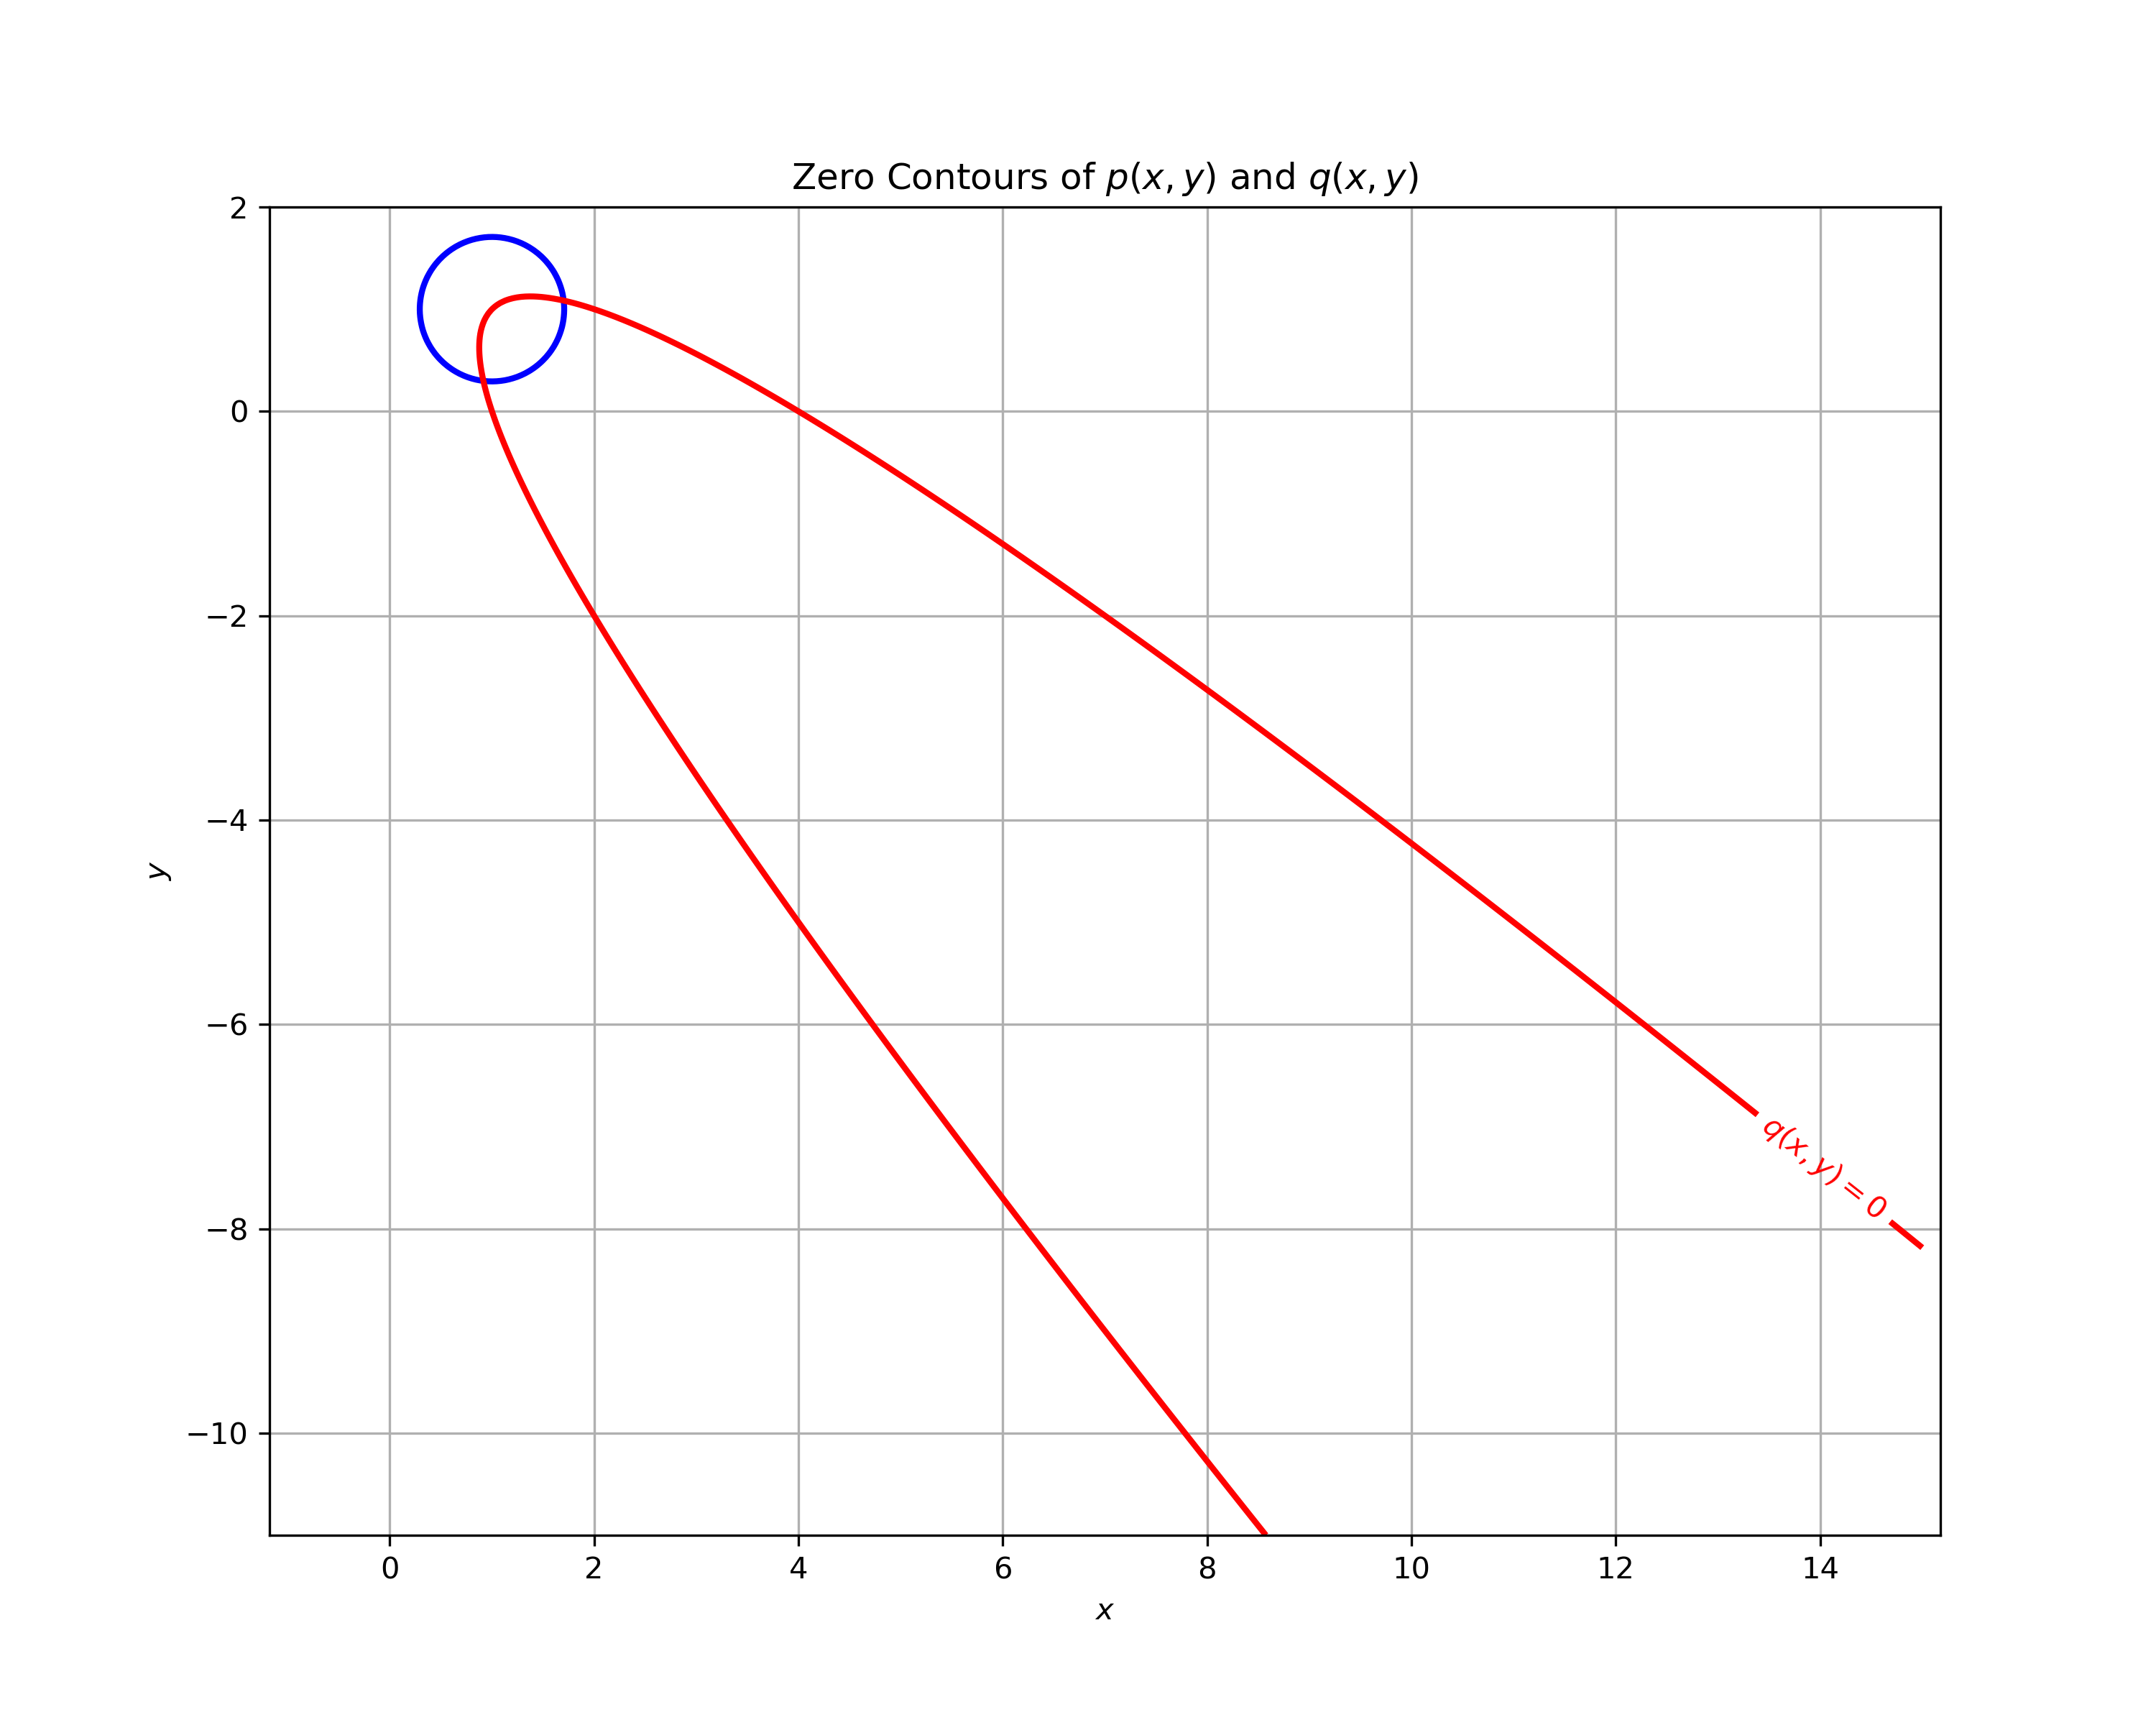
\includegraphics[width=.99\linewidth]{figs/zero_contour_both.png}
                            \caption{Zero Contour of $p(x, y) = 0$ and $q(x, y) = 0$}
                        \end{subfigure}
                        \begin{subfigure}{.49\linewidth}
                            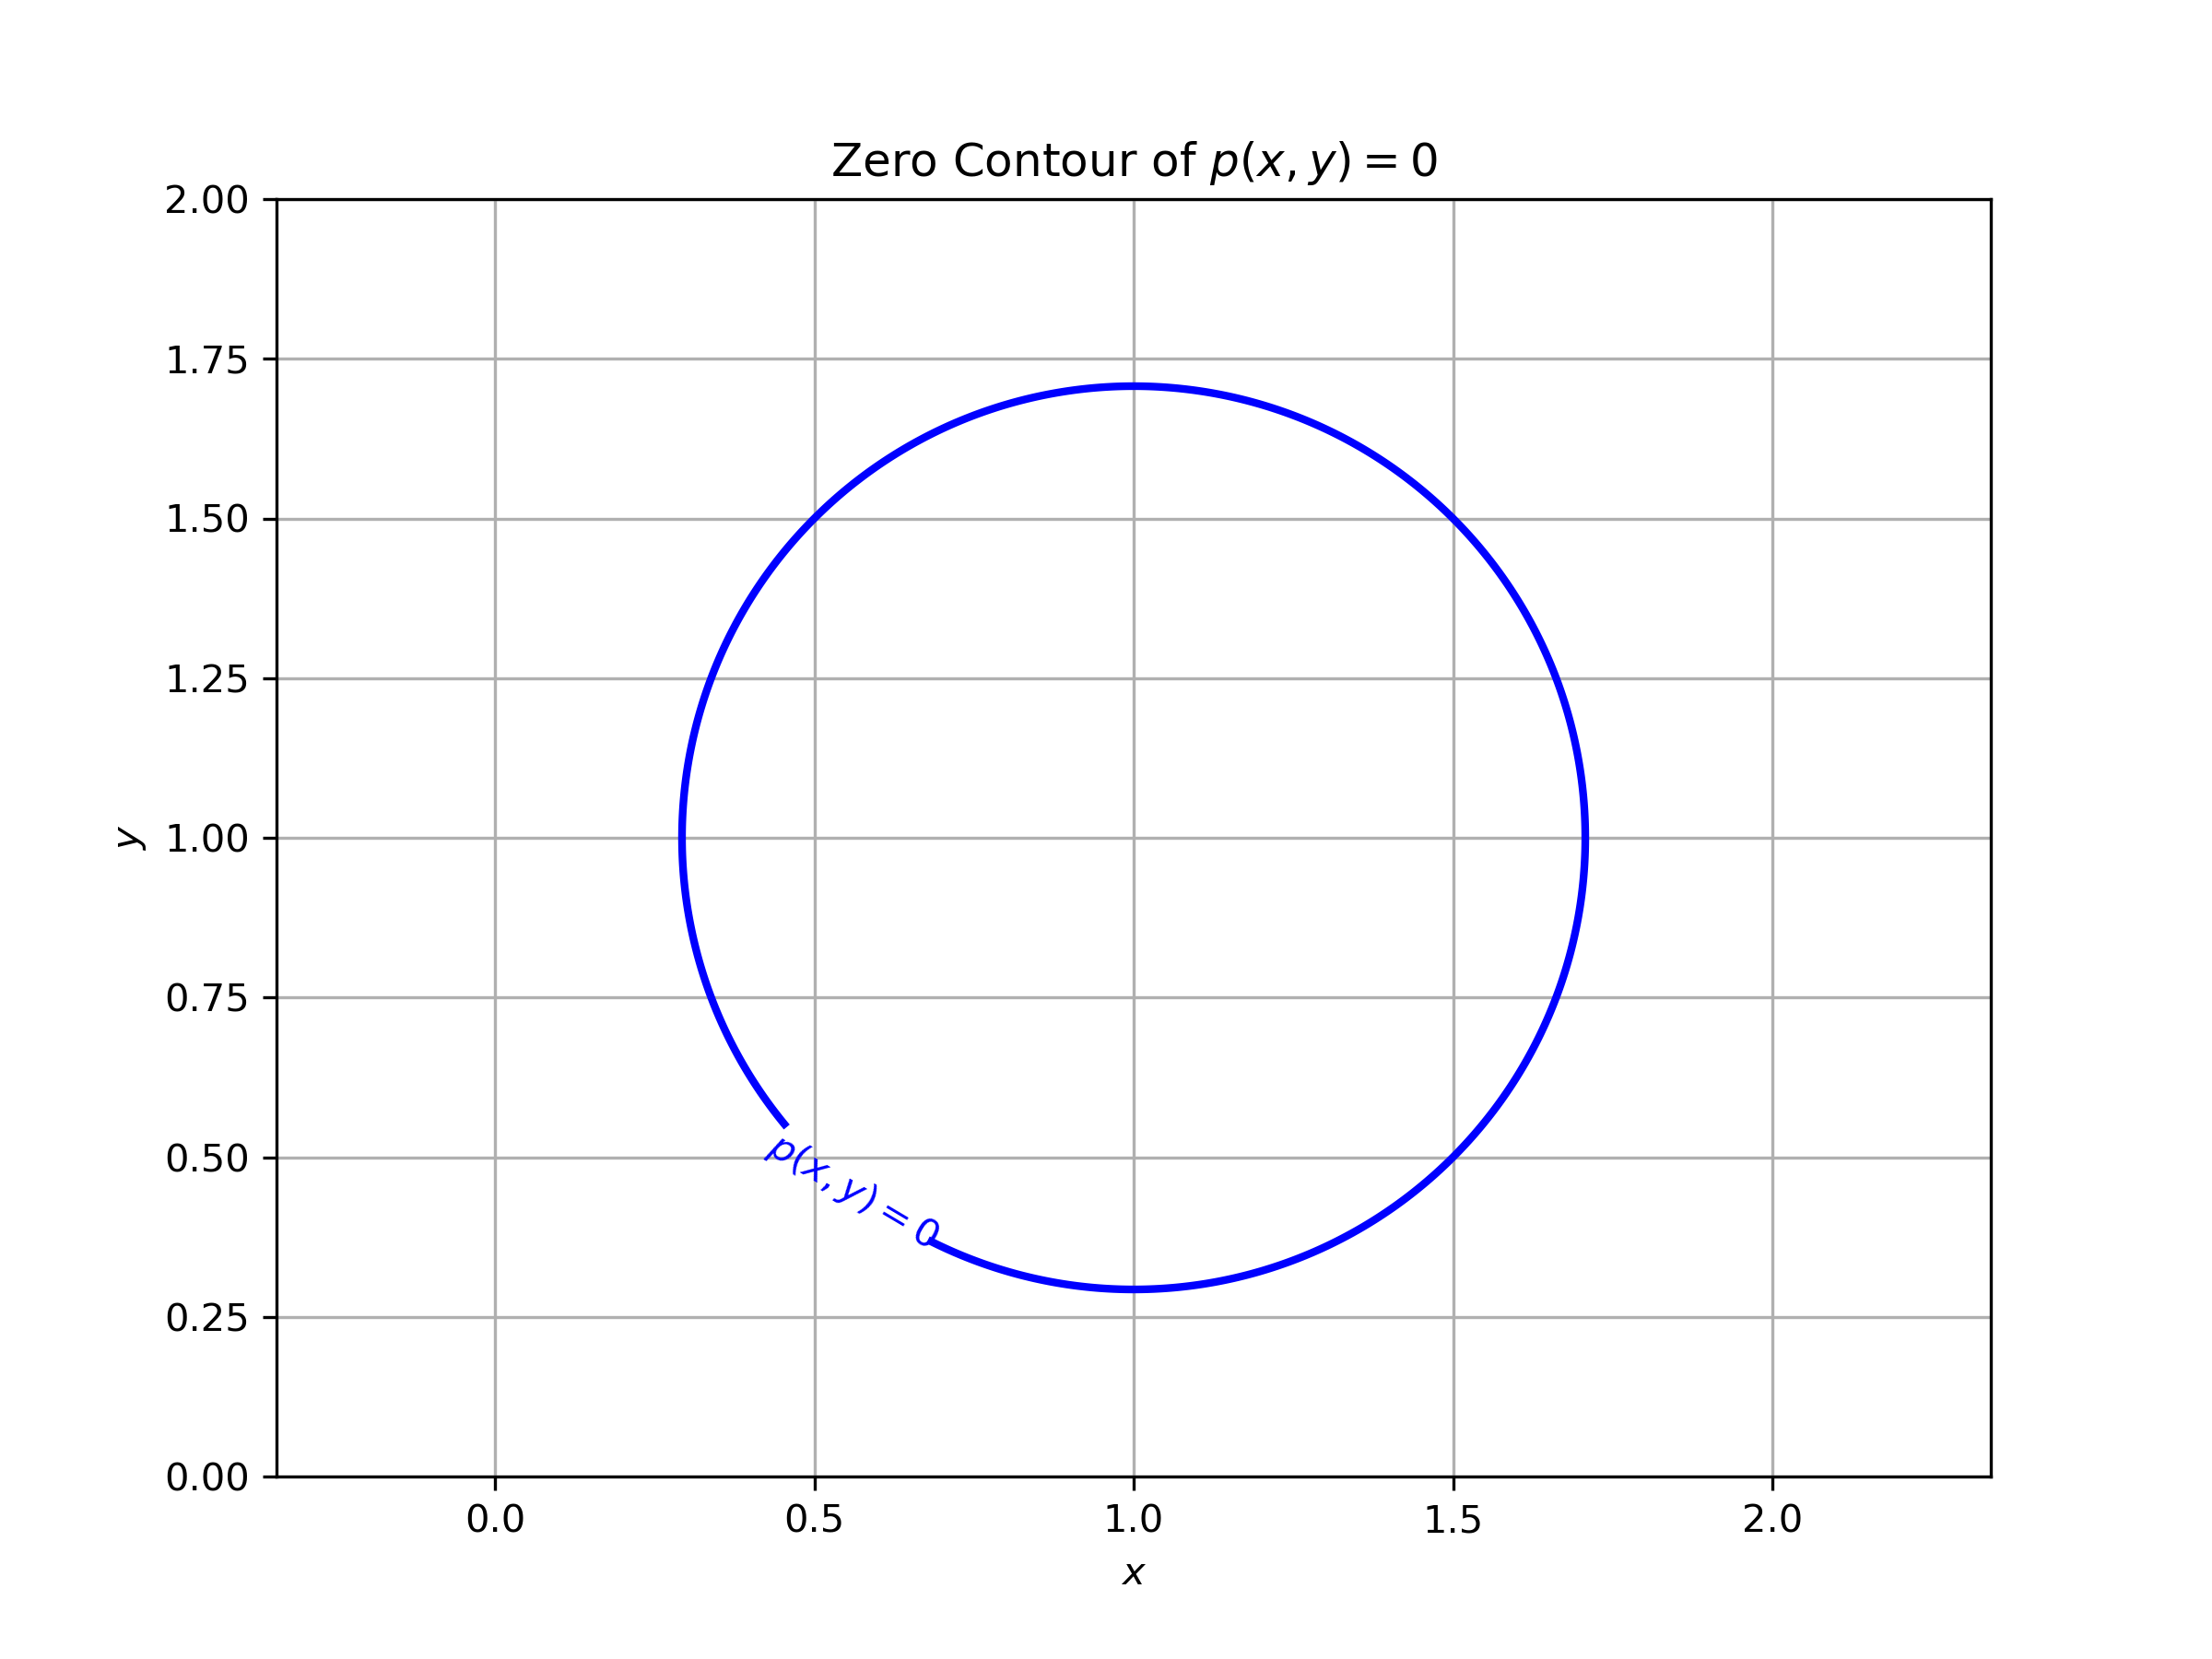
\includegraphics[width=.99\linewidth]{figs/zero_contour_p.png}
                            \caption{Zero Contour of $p(x, y) = 0$}
                        \end{subfigure}
                        \begin{subfigure}{.49\linewidth}
                            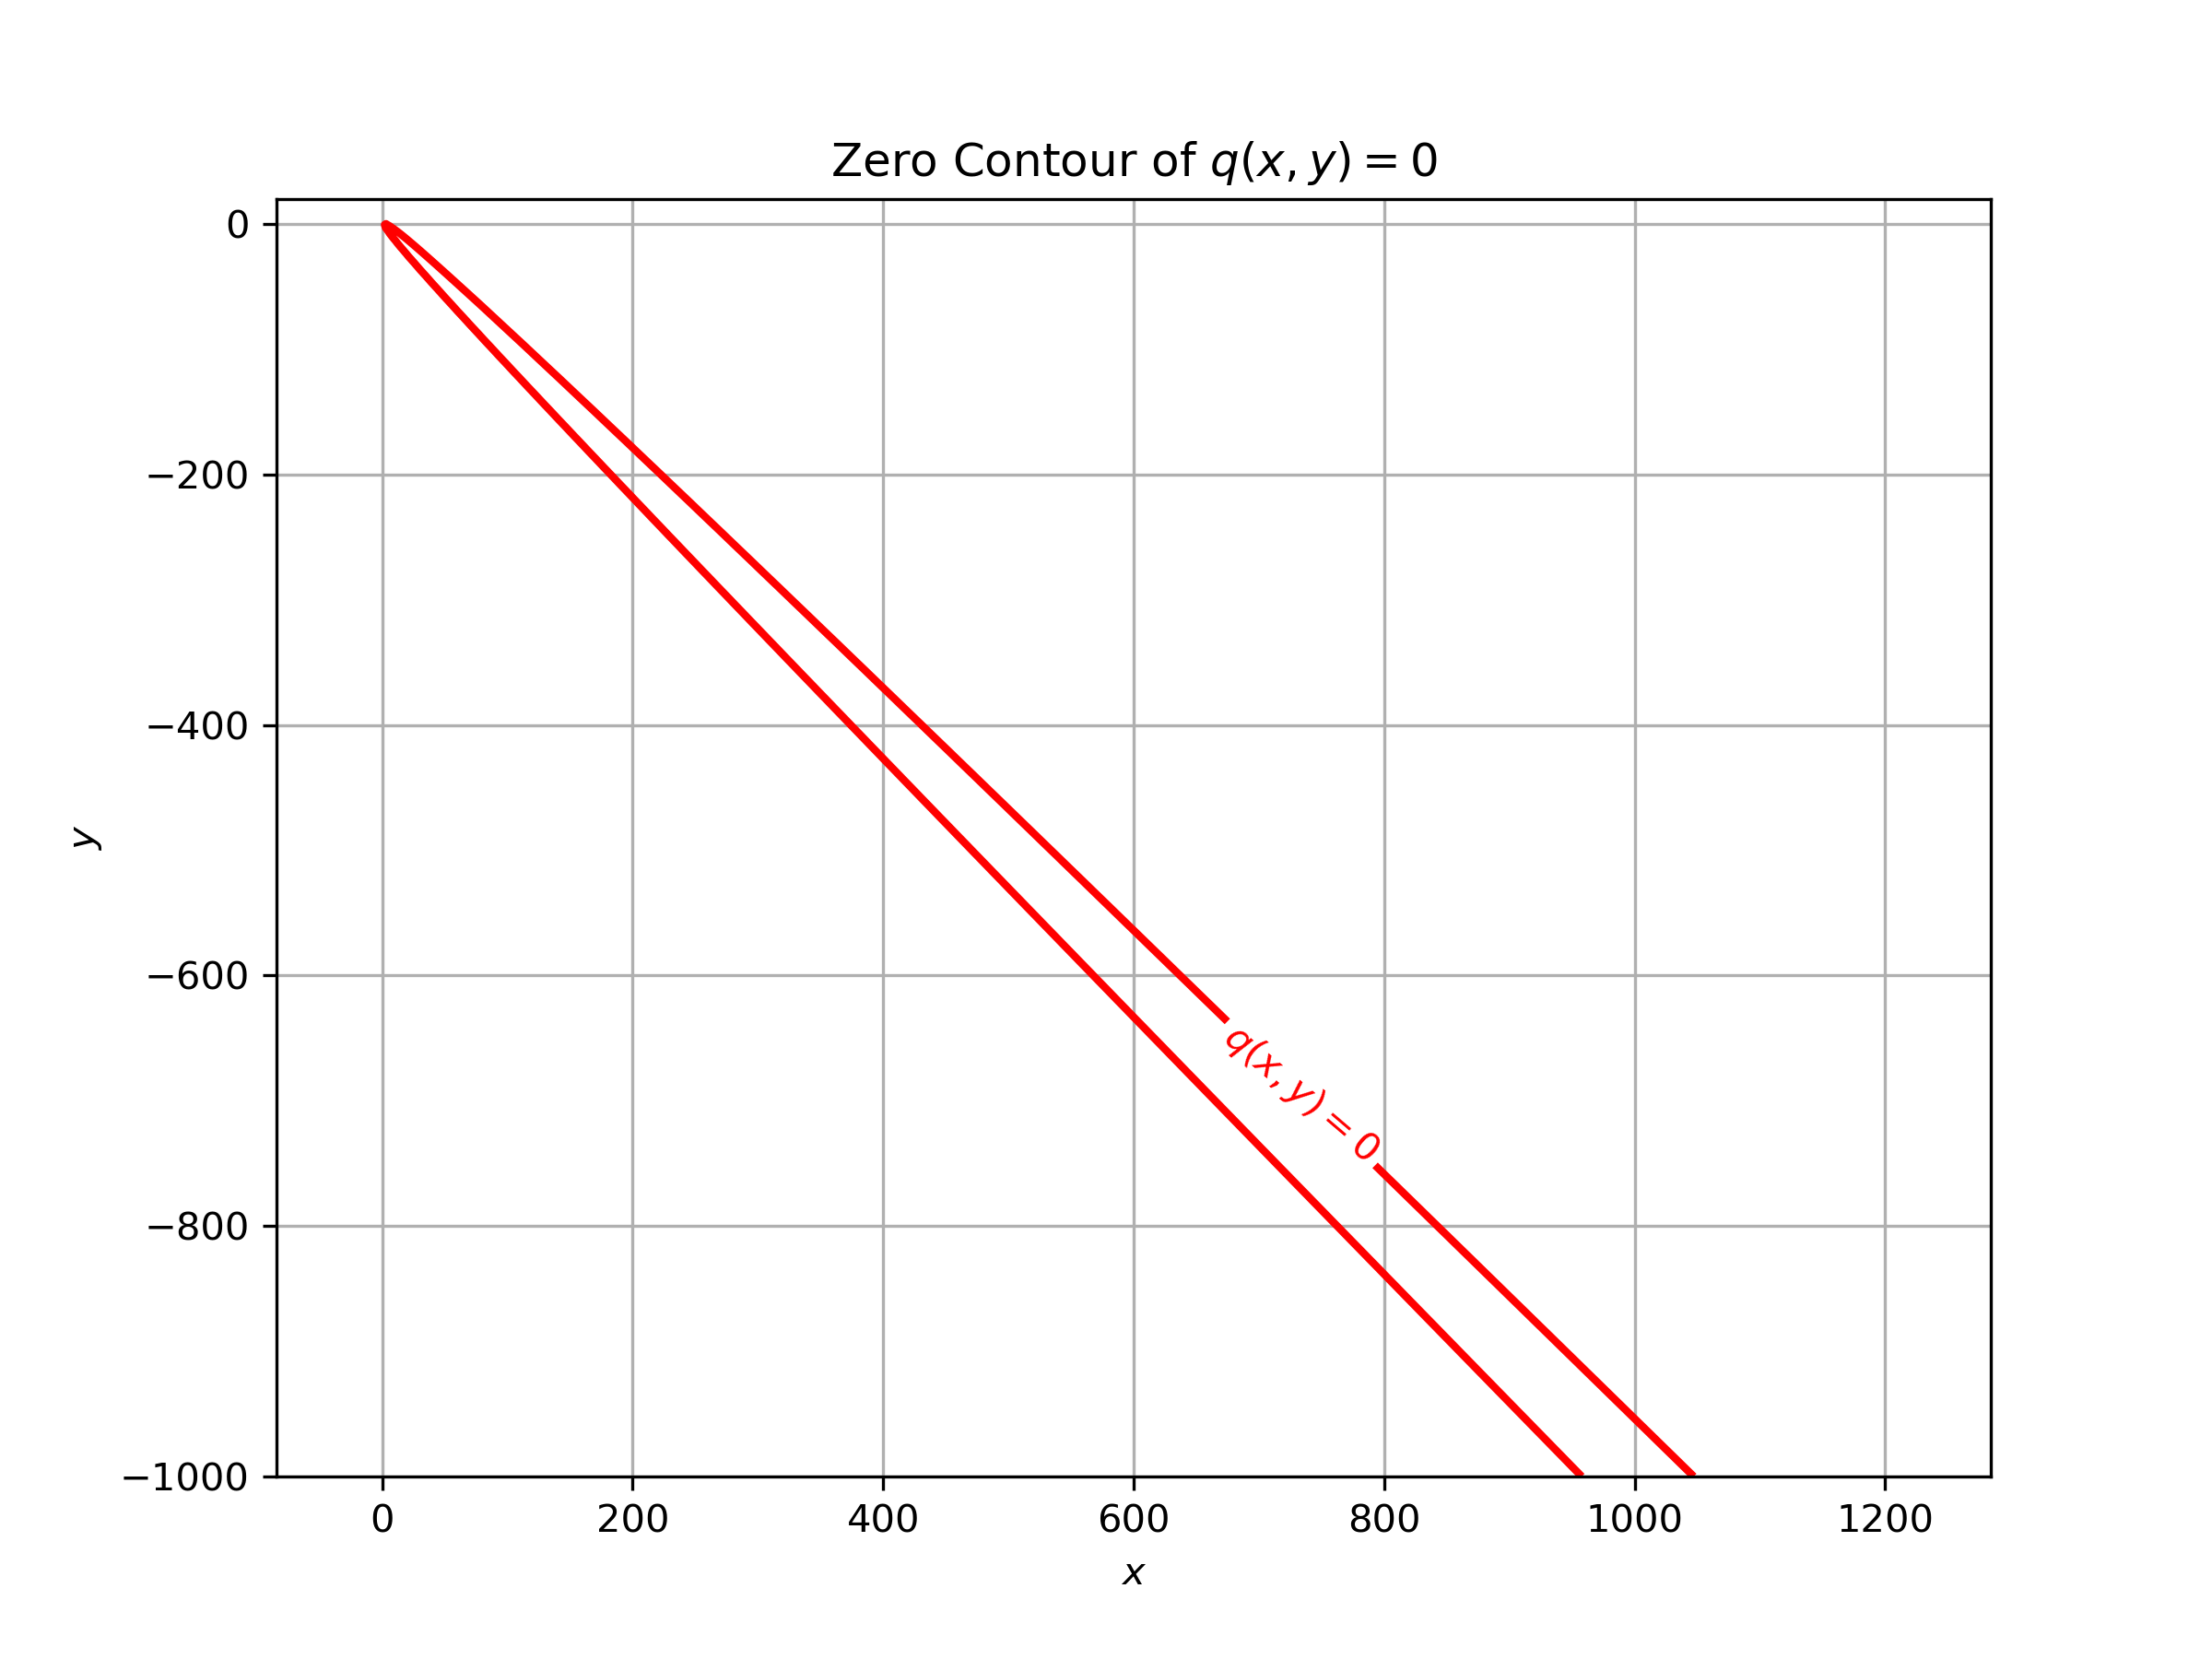
\includegraphics[width=.99\linewidth]{figs/zero_contour_q.png}
                            \caption{Zero Contour of $q(x, y) = 0$}
                        \end{subfigure}
                        \caption{\textbf{Zero Contours}}
                    \end{figure}

              \item Using the method of resultants, solve for the intersection points of these contours, i.e., find all (x, y) for which $p(x, y) = 0 = q(x, y)$, with x and y real.
                    Do so by treating the polynomials p and q as functions of y, temporarily viewing x as a constant.
                    Obtain a $4 \times 4$ matrix whose determinant, now a function of x, is the desired resultant.
                    Find the x-roots of that determinant, thereby projecting the intersection points onto the x-axis.
                    Use those x-roots to find the y-coordinates of the intersection points.
                    Verify your intersection points.

                    \textbf{Solution:}

                    Rewriting p and q as functions of y:
                    \begin{align*}
                        p(x, y) & = 2 x^2 + 2 y^2 - 4x - 4y + 3      \\
                        p(y)    & = 2 y^2 - 4y + (2 x^2 - 4x + 3)    \\
                        q(x, y) & = x^2 + y^2 + 2xy - 5x - 3y + 4    \\
                        q(y)    & = y^2 + (2x - 3)y + (x^2 - 5x + 4)
                    \end{align*}
                    Construct a $4 \times 4$ resultant matrix:
                    \begin{align*}
                        A      & =
                        \begin{bmatrix}
                            2 & -4     & 2 x^2 - 4x + 3 & 0              \\
                            0 & 2      & -4             & 2 x^2 - 4x + 3 \\
                            1 & 2x - 3 & x^2 - 5x + 4   & 0              \\
                            0 & 1      & 2x - 3         & x^2 - 5x + 4
                        \end{bmatrix}                          \\
                        det(A) & = 16 x^4 - 48 x^3 + 48 x^2 - 28 x + 11 = 0
                    \end{align*}

                    Substituting into the original $p(x, y)$ and $q(x, y)$, then solve for their common roots (\textit{in resultant.ipynb}), we have the following result
                    \begin{align*}
                        \begin{pmatrix}
                            x_1 \\
                            y_1
                        \end{pmatrix} & = \begin{pmatrix}
                            -\frac{\sqrt{5}}{4} + \frac{3}{4} - \sqrt{-\frac{\sqrt{5}}{8} - \frac{1}{8}} \\
                            \frac{\frac{3 \cdot \sqrt{2 + 2 \cdot \sqrt{5}}}{2} - \frac{3 \cdot \sqrt{5} \cdot i}{2} - \frac{i}{2}}{\sqrt{2} \cdot \sqrt{1 + \sqrt{5}} - \sqrt{5} \cdot i + i}
                        \end{pmatrix} \approx
                        \begin{pmatrix}
                            0.190983005625053 - 0.636009824757034 \cdot i \\
                            1.80901699437495 - 0.636009824757034 \cdot i
                        \end{pmatrix}                                        \\
                        \begin{pmatrix}
                            x_2 \\
                            y_2
                        \end{pmatrix} & = \begin{pmatrix}
                            -\frac{\sqrt{5}}{4} + \frac{3}{4} + \sqrt{-\frac{\sqrt{5}}{8} - \frac{1}{8}} \\
                            \frac{\frac{3 \cdot \sqrt{2 + 2 \cdot \sqrt{5}}}{2} + \frac{3 \cdot \sqrt{5} \cdot i}{2} + \frac{i}{2}}{\sqrt{2} \cdot \sqrt{1 + \sqrt{5}} + \sqrt{5} \cdot i - i}
                        \end{pmatrix} \approx
                        \begin{pmatrix}
                            0.190983005625053 + 0.636009824757034 \cdot i \\
                            1.80901699437495 + 0.636009824757034 \cdot i
                        \end{pmatrix}                                        \\
                        \begin{pmatrix}
                            x_3 \\
                            y_3
                        \end{pmatrix} & = \begin{pmatrix}
                            \frac{\sqrt{5}}{4} + \frac{3}{4} - \sqrt{\frac{\sqrt{5}}{8} - \frac{1}{8}} \\
                            \frac{-\frac{3 \cdot \sqrt{-2 + 2 \cdot \sqrt{5}}}{2} + \frac{3 \cdot \sqrt{5}}{2} - \frac{1}{2}}{-\sqrt{2} \cdot \sqrt{-1 + \sqrt{5}} + \sqrt{5} + 1}
                        \end{pmatrix} \approx
                        \begin{pmatrix}
                            0.915941305496236 \\
                            0.297907316746341
                        \end{pmatrix}                                        \\
                        \begin{pmatrix}
                            x_4 \\
                            y_4
                        \end{pmatrix} & = \begin{pmatrix}
                            \frac{\sqrt{5}}{4} + \frac{3}{4} + \sqrt{\frac{\sqrt{5}}{8} - \frac{1}{8}} \\
                            \frac{\frac{3 \cdot \sqrt{-2 + 2 \cdot \sqrt{5}}}{2} + \frac{3 \cdot \sqrt{5}}{2} - \frac{1}{2}}{\sqrt{2} \cdot \sqrt{-1 + \sqrt{5}} + \sqrt{5} + 1}
                        \end{pmatrix} \approx
                        \begin{pmatrix}
                            1.70209268325366 \\
                            1.08405869450376
                        \end{pmatrix}
                    \end{align*}
          \end{enumerate}

          \clearpage
    \item You are preparing a robotic unicycle to take part in a circus act.
          For most of the show, a talented acrobat rides the unicycle.
          But at one point, the acrobat jumps off the unicycle onto a trapeze.
          After a short trapeze act, the acrobat leaps through the ring of fire in the center of the stage to land on the waiting unicycle, which has moved autonomously to the other side.
          Your job is to plan a path for the unicycle to take around the ring of fire to the acrobat's landing point.

          You are given a precomputed set of paths which all begin at different points, avoid the ring of fire, and end at the destination (shown below).
          You must mimic these paths as closely as possible, since they are precisely choreographed for the circus act.
          However, the acrobat is only human, and does not position the unicycle precisely at any of the paths' starting points.

          You will need to interpolate a new path from other paths with nearby starting points.

          \begin{figure}[H]
              \centering
              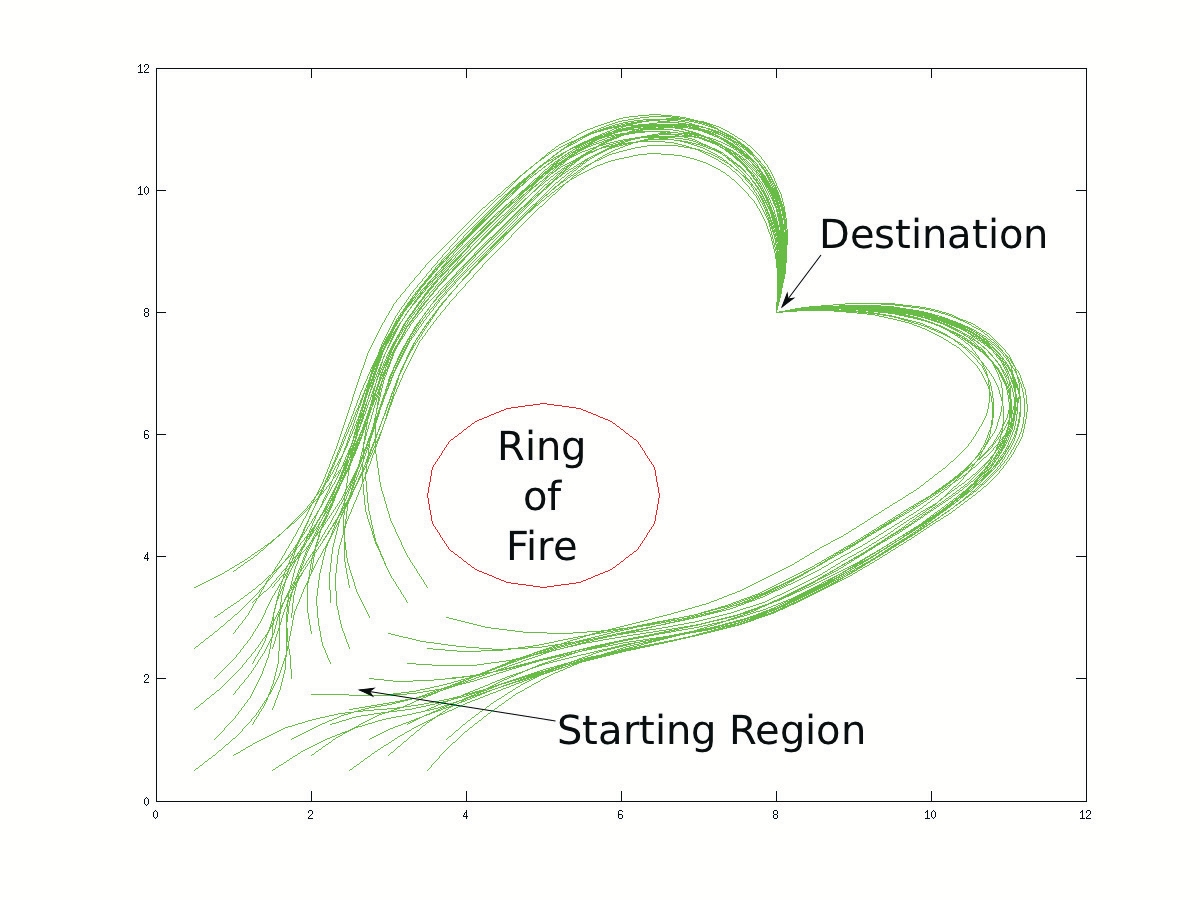
\includegraphics[width=.8\linewidth]{figs/Q8.jpg}
              \caption{Unicycle Path Planning}
          \end{figure}

          The Destination point is (8, 8). The Ring of Fire is a circle of radius 1.5 centered at (5, 5).

          The precomputed paths are given in the text file paths.txt.
          Every pair of lines in the text file represents a path, which is a sequence of 50 points.
          The first line contains the x coordinates, and the second contains the y coordinates for one path.
          The file format is:
          \begin{align*}
              \begin{matrix}
                  x_0^{(1)} & x_1^{(1)} & \ldots & x_{48}^{(1)} & x_{49}^{(1)} \\
                  y_0^{(1)} & y_1^{(1)} & \ldots & y_{48}^{(1)} & y_{49}^{(1)} \\
                  x_0^{(2)} & x_1^{(2)} & \ldots & x_{48}^{(2)} & x_{49}^{(2)} \\
                  y_0^{(2)} & y_1^{(2)} & \ldots & y_{48}^{(2)} & y_{49}^{(2)} \\
                  \ldots    & \ldots    & \ldots & \ldots       & \ldots
              \end{matrix}
          \end{align*}
          \begin{center}
              (Notation: the superscripts (1), (2), $\ldots$ are path indices, not derivatives.)
          \end{center}

          \begin{enumerate}
              \item Write a system of linear equations (in the form $Av = b$, with $v$ representing variables of some sort, appropriately chosen) and constraints (for instance, $v_1 \leq 0$) that will help you determine whether a 2D point (x, y) falls within the triangle formed by three 2D points $(x^{(i)}, y^{(i)})$, $(x^{(j)}, y^{(j)})$, and $(x^{(k)}, y^{(k)})$.
                    (Part of the problem is to think about how you might do this.)

                    \textbf{Solution:}

                    Convexity.

                    The three 2D points $(x^{(1)}, y^{(1)})$, $(x^{(2)}, y^{(2)})$, and $(x^{(3)}, y^{(3)})$ form a triangle, which is a convex polygon.

                    Recall that for all points $p$ in a convex polygon with vertices $v_1, v_2, \ldots, v_n$, the following inequality holds:
                    \begin{align*}
                        \sum_{i=1}^{n} \lambda_i v_i  & = p,                  \\
                        s.t. \sum_{i=1}^{n} \lambda_i & = 1, \lambda_i \geq 0
                    \end{align*}
                    So we can form a system of linear equations with constraints:
                    \begin{align*}
                        \begin{bmatrix}
                            x^{(1)} & x^{(2)} & x^{(3)} \\
                            y^{(1)} & y^{(2)} & y^{(3)}
                        \end{bmatrix} \cdot
                        \begin{pmatrix}
                            \lambda_1 \\
                            \lambda_2 \\
                            \lambda_3
                        \end{pmatrix}             & =
                        \begin{pmatrix}
                            x \\
                            y
                        \end{pmatrix}                                     \\
                        s.t. \lambda_1 + \lambda_2 + \lambda_3 & = 1, \lambda_i \geq 0
                    \end{align*}
                    This can be further simplified to
                    \begin{align*}
                        \begin{bmatrix}
                            x^{(1)} & x^{(2)} & x^{(3)} \\
                            y^{(1)} & y^{(2)} & y^{(3)} \\
                            1       & 1       & 1
                        \end{bmatrix} \cdot
                        \begin{pmatrix}
                            \lambda_1 \\
                            \lambda_2 \\
                            \lambda_3
                        \end{pmatrix} & =
                        \begin{pmatrix}
                            x \\
                            y \\
                            1
                        \end{pmatrix}     \\
                        s.t. \lambda_i \geq 0
                    \end{align*}
              \item Implement an algorithm to create a path for the unicycle as follows:

                    [Notation: For a path p, p(t) is the 2D point $(x^{(t)}, y^{(t)})$ that describes the location of the path at time t.
                    Exactly what time scale you choose is up to you, so long as the unicycle's motion starts at time t = 0.]

                    \begin{itemize}
                        \item Assume the algorithm is given the unicycle's starting location at time t = 0.
                        \item Your algorithm should first pick three paths $p^{(i)}$, $p^{(j)}$, and $p^{(k)}$ (from the file paths.txt), subject to some constraints described next.
                        \item The three paths should all lie on the same side of the ring of fire, all passing either to the left or all to the right of the ring.
                        \item Your algorithm should construct a new path p as a weighted sum of these three paths.
                              So, at each time t, $p(t) = \alpha_i p^{(i)}(t) + \alpha_j p^{(j)}(t) + \alpha_k p^{(k)}(t)$, with p(0) the given starting location of the unicycle and with the weights $\alpha_i$, $\alpha_j$, $\alpha_k$ fixed throughout.
                        \item You should choose these weights so that p(0) lies within the triangle formed by the starting locations of the three paths that your algorithm picks, that is, within the triangle formed by the points $p^{(i)}(0)$, $p^{(j)}(0)$, and $p^{(k)}(0)$.
                        \item Your algorithm should be able to produce a value p(t) for all relevant (continuous) times t prior to reaching the Destination, not just for the discrete time snapshots given in paths.txt.
                              (It is here that interpolation comes into play.
                              Use whatever interpolation method you find useful.
                              Something simple is fine.)
                        \item At all times, p(t) should lie outside the ring of fire.
                    \end{itemize}

                    Comment: The unicycle's starting position should fall within the triangle formed by three paths' starting points, but there may be many valid such triples of paths.
                    (You may assume there is at least one.)
                    You should develop your own criteria for choosing one such triple of paths, $p^{(i)}$, $p^{(j)}$, $p^{(k)}$.

                    Specificity: You only need to write code to solve the particular problem (with the particular destination, ring of fire, and precomputed paths) described here, not a general purpose algorithm.

                    \textbf{Solution:}

                    \begin{lstlisting}[language=Python]
def above_line(P: np.ndarray, P0: np.ndarray, P1: np.ndarray) -> bool:
    """Return True if P is above the line P0 --- P1, False otherwise

    Args:
        P (np.ndarray): 2 x 1 2D point
        P0 (np.ndarray): 2 x 1 2D point
        P1 (np.ndarray): 2 x 1 2D point

    Returns:
        bool: True if P is above the line P0 --- P1, False otherwise
    """

    x0, y0 = P0
    x1, y1 = P1
    x, y = P

    return (y - y0) * (x1 - x0) - (x - x0) * (y1 - y0) > 0
                    \end{lstlisting}
                    \begin{lstlisting}[language=Python]
def out_of_circle(P: np.ndarray):
    """Return True if P(s) outside the circle, False otherwise

    Args:
        P (np.ndarray): must be of shape 2 x n
    """

    # Circle center
    center = np.array([[5], [5]])

    # Circle radius
    r = 1.5

    # Check if P is outside the circle
    return np.linalg.norm(P - center, axis=0) > r
                    \end{lstlisting}
                    \begin{lstlisting}[language=Python]
# Remove any paths that have points inside the ring of fire
safe_paths = []

for path in paths:
    if not np.any(~out_of_circle(path)):
        safe_paths.append(path)

paths = np.array(safe_paths)

# Categorize the path into above or below the ring of fire
above = []
below = []

for path in paths:
    # Check if the center point of a path is above or below the line formed by connecting starting and ending points
    center = np.average(path, axis=1)

    if above_line(center, path[:, 0], path[:, -1]):
        above.append(path)
    else:
        below.append(path)

above = np.array(above)
below = np.array(below)
                    \end{lstlisting}
                    \begin{lstlisting}[language=Python]
def select_paths(P: np.ndarray) -> np.ndarray:
    """Select 3 paths from the given paths in either above or below whose starting points surround the input starting point

    Args:
        P (np.ndarray): starting point in shape 2 x 1

    Returns:
        np.ndarray: shape 3 x 2 x 50
    """

    above_tri = Delaunay(above[:, :, 0])
    below_tri = Delaunay(below[:, :, 0])

    # Find the triangle that contains the starting point
    simplex = above_tri.find_simplex(P.T)

    if simplex == -1:
        simplex = below_tri.find_simplex(P.T)

        if simplex == -1:
            raise ValueError("Starting point not found in any triangle")

        else:
            vertices = below_tri.simplices[simplex]

            return below[*vertices]
    else:
        vertices = above_tri.simplices[simplex]

        return above[*vertices]
    # unpack because vertices is wrapped twice
                    \end{lstlisting}
                    \begin{lstlisting}[language=Python]
# Solve alpha_i, alpha_j, alpha_k

# Construct A
A = path_starting_points.T  # Shape: (2, 3)

# Append the row [1, 1, 1] to A
A_aug = np.vstack((A, np.ones((1, 3))))

# Construct b_aug
b_aug = np.append(initial_point, 1)

# Solve the linear system with constraints
# Since lambda_i >= 0, we can use a constrained optimization solver
# Objective function (arbitrary since we only need feasible solution)
c = np.zeros(3)

# Inequality constraints: lambda_i >= 0
bounds = [(0, None), (0, None), (0, None)]

# Equality constraints: A_aug @ lambda = b_aug
res = linprog(c, A_eq=A_aug, b_eq=b_aug, bounds=bounds, method='highs')

if res.success:
    alphas = res.x
else:
    print("Failed to compute weights.")
    # Handle this case
                    \end{lstlisting}
                    \begin{lstlisting}[language=Python]
# Weighted average of the paths
path = np.sum(np.multiply(selected_paths, alphas[:, None, None]), axis=0)

time_step = np.linspace(0, path.shape[1] - 1, path.shape[1])

# Interpolate with Spline
p_x = UnivariateSpline(time_step, path[0], s=0)
p_y = UnivariateSpline(time_step, path[1], s=0)

# Construct p(t)
def p(t):
    return np.array([[p_x(t)], [p_y(t)]])
                    \end{lstlisting}

                    Refer to my code in \textit{unicycle\_path\_planning.ipynb} for the complete implementation with result verification.
              \item Discuss any decisions you made in your implementation, for example: How did you pick the triple of paths $p^{(i)}$, $p^{(j)}$, $p^{(k)}$?
                    How did you choose the weights $\alpha_i$, $\alpha_j$ , $\alpha_k$?
                    How did you decide on a time scale for t?
                    How did you decide on an interpolation method?

                    \textbf{Solution:}

                    \begin{itemize}
                        \item All the input paths will be categorized into above/below the ring of fire
                        \item 3 Paths are picked based on the Delaunay triangulation of the starting points of the paths, if the input initial point falls within a triangle, the paths forming the triangle will be selected
                        \item Weights are computed by solving a linear system with convexity constraints
                        \item Time scale is set to $[0, \text{\# interpolation points} - 1]$ for simplicity
                        \item Spline interpolation is used for smooth path interpolation and simplicity, I set $k = 5$ for smoothness analogous to minimum jerk/snap trajectory for easier control.
                    \end{itemize}
                    Refer to my code in \textit{unicycle\_path\_planning.ipynb} for more detailed answer to these questions with annotation.
              \item Interpolate paths for the starting points (0.8, 1.8), (2.2, 1.0) and (2.7, 1.4).
                    For each starting point, on the same graph, plot the ring of fire, the three paths being interpolated, and the interpolated path.
                    The paths should not touch the ring of fire.

                    \textbf{Solution:}

                    \begin{figure}[H]
                        \centering
                        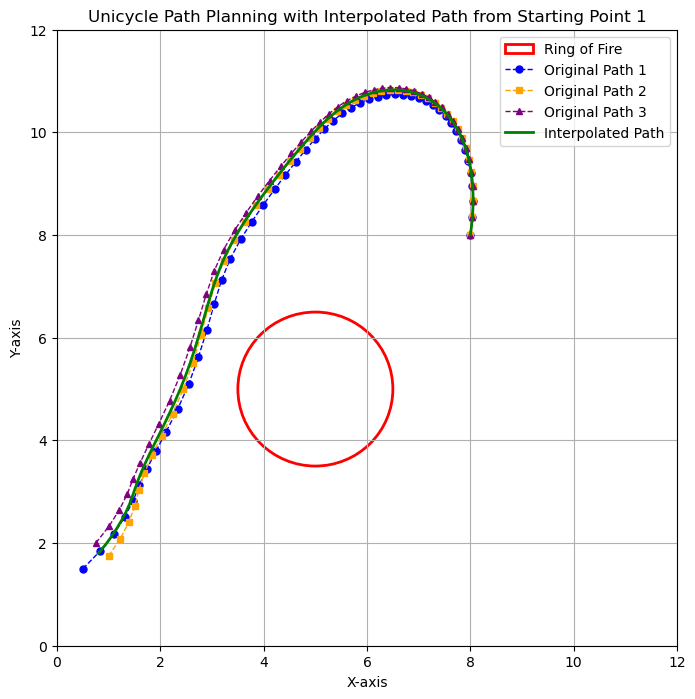
\includegraphics[width=.99\linewidth]{"figs/Q8_path_1.png"}
                        \caption{Interpolated Path for Starting Point (0.8, 1.8)}
                    \end{figure}

                    \begin{figure}[H]
                        \centering
                        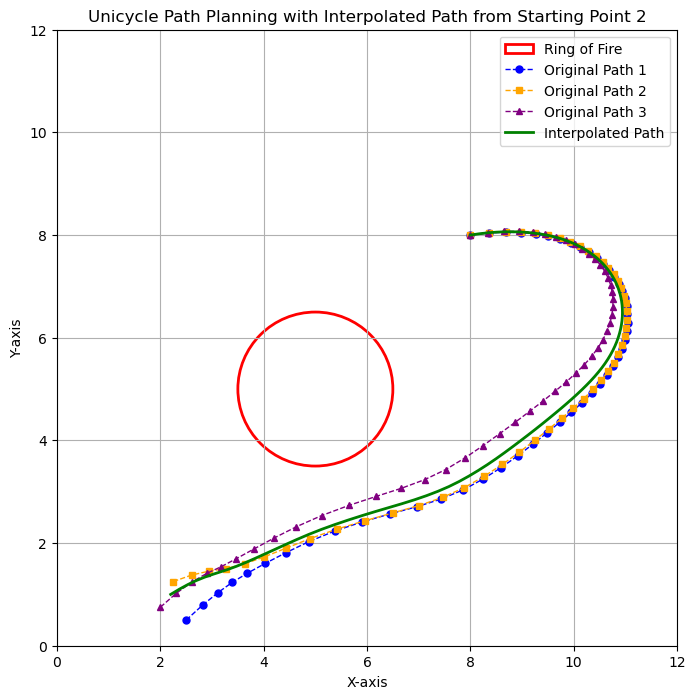
\includegraphics[width=.99\linewidth]{"figs/Q8_path_2.png"}
                        \caption{Interpolated Path for Starting Point (2.2, 1.0)}
                    \end{figure}

                    \begin{figure}[H]
                        \centering
                        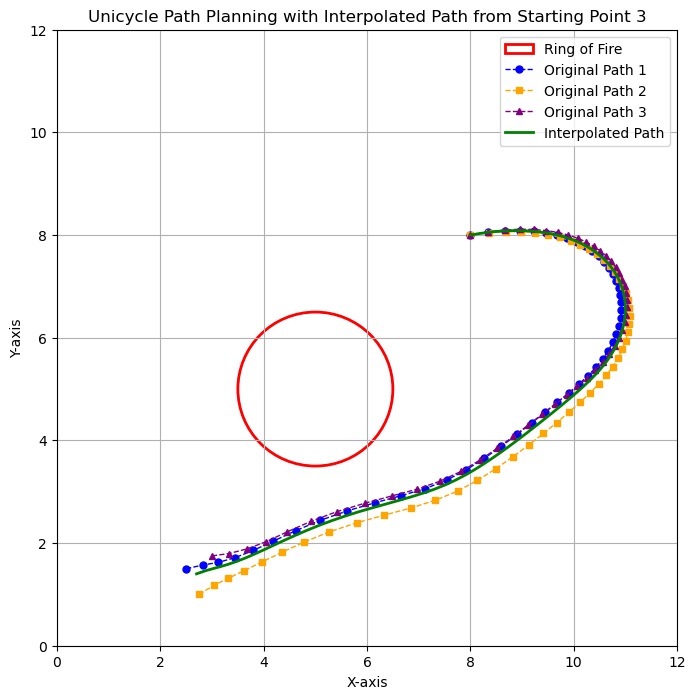
\includegraphics[width=.99\linewidth]{"figs/Q8_path_3.png"}
                        \caption{Interpolated Path for Starting Point (2.7, 1.4)}
                    \end{figure}
              \item Discuss how your algorithm would need to be modified (if at all) if more obstacles like the ring of fire were to be introduced.

                    \textbf{Solution:}

                    Add more pre-processing steps to discard input paths that intersect with the new obstacles.
                    For safety guarantees, we can interpolate all the input paths with the same interpolation function to see if the continuous path curve intersect with the new obstacles.

                    This will work as long as the selected paths are not intersecting with the new obstacles, because the new interpolated path will always fall within the tube formed by the selected paths.
          \end{enumerate}
\end{enumerate}

\end{document}
